\documentclass[11pt,a4paper]{article}

\usepackage[margin=2.3cm]{geometry}
\usepackage{amsmath,amssymb}
\usepackage{graphicx}
\usepackage{booktabs}
\usepackage{xcolor}
\usepackage{enumitem}
\usepackage[hidelinks]{hyperref}
\usepackage{caption}

\emergencystretch=3em
\captionsetup{font=small,labelfont=bf,width=.92\textwidth}
\setlength{\parskip}{4pt plus 1pt}
\setlength{\parindent}{0pt}

\newcommand{\code}[1]{\texttt{#1}}
\newcommand{\Kp}{K'}
\newcommand{\TopK}{\operatorname{TopK}}
\newcommand{\sgn}{\operatorname{sign}}
\newcommand{\sg}{\operatorname{sg}}
\newcommand{\PH}[1]{\textcolor{red}{[#1]}}

\title{Laplace-policy hard Top-$K$ under the code residual:\\
why the likelihood-ratio estimator fails, and a Rao--Blackwellized fix\\[2pt]
\large Research note: calibration, diagnosis and repair of \code{surrogate\_mode: laplace\_policy}}
\author{}
\date{2026-10-08.}

\begin{document}
\maketitle
\vspace{-2em}

% ============================================================
\section{Purpose and summary of conclusions}
% ============================================================

\code{laplace\_policy} trains an exactly $K$-sparse bottleneck whose training
forward keeps $K$ members of the clean Top-$(K{+}J)$ pool chosen by
Laplace-perturbed scores; the selection is trained with the likelihood-ratio
(score-function) estimator of the expected sampled cross-entropy
(\code{docs/laplace-policy-topk.md}). This note began as a temperature
campaign on four cells of the code-carried K+J grid of
\code{docs/kj-vs-hard-topk-code-residual.tex} -- a constant against an
exponentially annealed noise width -- and became a diagnosis: after 2500 steps
every one of the eight campaign runs was at the unigram level of the loss
(clean validation CE $5.95$--$6.09$, against $1.89$ for RBLapSum $T=2$ at the
same step), and the campaign was stopped to find the cause.

The main conclusions are:

\begin{itemize}[leftmargin=1.4em]
\item \textbf{An absolute noise width cannot be calibrated at step 30.} With
$T$ chosen so that $15$--$20\%$ of the sampled support is exchanged at step 30,
the exchange falls below $3\%$ in every cell by step 200, because the pool's
score span grows about tenfold between steps 50 and 200 in every policy probe,
at every width; the hard and RBLapSum models keep theirs, and so does the same
sampled forward without the selection term. The growth is the selection
gradient's push along the score scale. A width proportional to the pool span
holds the exchange; the campaign used it.

\item \textbf{The likelihood-ratio estimator is noise.} Per sequence it is one
advantage times the sum of $8 \times 512 \times (K{+}J) \approx 2 \times 10^6$
log-density gradients of $\pm 1/T$ each, while only boundary crossings carry
signal. On a fixed batch and checkpoint the per-draw noise of the selection
gradient is $6.7 \times 10^3$--$3.7 \times 10^4$ in norm against $0.35$--$1.13$
for the value gradient, and the Monte Carlo signal is not resolved with 64
draws. Clipped to norm 1 on every step, the update is a unit-norm random
direction; the same model with the selection term removed ($\gamma = 0$) trains
like the references (validation CE $2.73$ at step 500 against $2.69$ for
RBLapSum).

\item \textbf{Rao--Blackwellization over each member's own noise removes that
variance.} The conditional expectation of the likelihood-ratio sample given all
other noise is the crossing density at the member's threshold times the loss
difference of the single swap it controls -- exact, baseline-free. Taking the
swap difference to first order from the backpropagated gradient gives an
estimator whose per-draw noise is of the order of the value gradient (signal
to noise $0.6$--$1.1$ per draw, against $0.01$--$0.1$).

\item \textbf{Two further conditions follow from the code residual and the
relative width.} Linearizing the swap with the total downstream gradient lets
selection terms multiply along the carry (gradient norms $5 \times 10^3$ to
$8.5 \times 10^5$ within 120 steps): the swap must be linearized along hard
paths only (first-order scope). And the frozen-width gradient of a relative width has a component along
the score scale that, followed with a low-noise estimator, made the pool span
grow from $13$ to $2.2 \times 10^5$ in 400 steps; removing that component
(orthogonal projection, which the exact gradient satisfies by Euler's identity)
fixes it without the noise of differentiating the span itself.

\item \textbf{With the three changes the method trains.} %%HEADLINE%%
\end{itemize}

% ============================================================
\section{Definitions}
% ============================================================

\paragraph{The gate.}
The model is the code-carried stack of \code{docs/kj-vs-hard-topk-code-residual.tex}:
$L = 8$ blocks of width $d = 768$, an abs-TopK bottleneck with $N = 1536$
features after every block, the $K$-sparse code carried from block 1 on, no
output norm. For one token at gate $\ell$, $z \in \mathbb{R}^N$ is the encoder
output and $s = |z|$ its scores. The clean pool is
$C = \operatorname{TopIndices}_{K+J}(s)$, sorted $s_{(1)} \ge \dots \ge s_{(K+J)}$;
the clean support is $S_{\mathrm{clean}} = \{(1), \dots, (K)\}$.

\paragraph{The sampled support.}
In training the gate keeps $K$ members of $C$ chosen by noisy scores,
\begin{equation}
u_i = s_i - \frac{1}{K+J}\sum_{j \in C} s_j, \qquad
r_i = u_i + \varepsilon_i, \quad \varepsilon_i \sim \mathrm{Laplace}(0, T), \qquad
S = \TopK_{i \in C}(r_i),
\label{eq:sample}
\end{equation}
and transmits the original values $v_i = z_i$ for $i \in S$. Evaluation uses
$S_{\mathrm{clean}}$. The objective is the expected sampled CE,
$\mathcal J_T = \mathbb E_\varepsilon[L(S)]$.

\paragraph{Width.}
$T_{\mathrm{abs}} = \tau$ or $T_{\mathrm{span}} = \tau\,(s_{(K+1)} - s_{(K+J)})$
per row (\code{policy\_temperature\_mode} \code{absolute} or
\code{relative\_span}), with $\tau$ constant or annealed
($\tau(t) = \tau_0\,0.2^{v(t)}$, $v = \operatorname{clip}((t-1000)/17000, 0, 1)$).

\paragraph{Exchange fraction.}
$q_\ell = 1 - |S_\ell \cap S_{\ell,\mathrm{clean}}| / K$, the share of the
sampled support outside the clean one, averaged over the tokens of a
micro-batch at gate $\ell$; $q = 0$ is the hard Top-$K$ forward.

\paragraph{The likelihood-ratio estimator.}
With $c_b$ the mean CE of sequence $b$, $w_b$ its share of the valid tokens and
$B$ an exponential moving average of the training CE (decay $0.99$), the
selection gradient of one micro-batch is
\begin{equation}
\hat g_{\mathrm{LR}} = \sum_b w_b\,(c_b - B) \sum_{\ell=1}^{8} \sum_{t=1}^{512}
\sum_{i \in C_{\ell t}} \frac{\sgn(r_{\ell t i} - u_{\ell t i})}{T_{\ell t}}\,
\nabla_\theta u_{\ell t i},
\label{eq:lr}
\end{equation}
added to the value gradient through the sampled hard masks (the original
implementation, \code{policy\_estimator: likelihood\_ratio}).

\paragraph{Losses reported.}
The \emph{clean} validation CE (\code{val/ce}) is the deterministic Top-$K$
forward, the quantity every comparison uses (RBLapSum and hard Top-$K$ train and
validate with a clean forward); the \emph{stochastic} one is the mean over
sampled draws. Both use 40 batches of $24 \times 512$ tokens. ``Value gradient''
$g_{\mathrm{value}}$ is the CE gradient through the clean hard masks.

% ============================================================
\section{Setup}
% ============================================================

Four cells of the code-carried grid, $(K, J) = (32, 32)$, $(32, 480)$,
$(128, 128)$, $(256, 256)$. Each config is the stable RBLapSum cell
\code{configs/cr\_kj/ma\_cr\_rbk\_k<K>\_j<J>\_t2.yaml} (\code{code\_residual: true},
\code{post\_norm: false}) with the gate's training rule replaced and nothing
else changed (\code{scripts/make\_policy\_cr\_configs.py} checks this field by
field; files in \code{configs/policy\_cr/}): $8 \times 768$, abs-TopK over
$N = 1536$, \code{residual\_out} at every block, magnitude--direction
decoupling, batch $96 \times 512$, 20k steps with the cosine schedule (500
warm-up steps, peak $6 \times 10^{-4}$), clipping at norm 1, seed 1337, bf16.
References: the RBLapSum $T=2$ cells \code{ma\_cr\_rbk\_k<K>\_j<J>\_t2} and the
hard baselines \code{ma\_cr\_hard\_k<K'>\_pnorm} (with output norm) of the
code-residual note, same card model.

Boxes: \code{vienna} (eight RTX 5090) for the calibration, the campaign and the
first diagnostics; \code{zurich} (one RTX 5090) for the probes and the repaired
runs. Preflight on \code{vienna}: the CPU suite, the GPU repro oracle
(\code{hard}, \code{lapsum}, \code{rbk} bit-identical between \code{feb74a8} and
\code{c81fe44}), a policy smoke with a resume (baseline and update count restored
from \code{policy\_state}), and \code{scripts/policy\_preflight.py} on every cell
(one policy record per gate, exactly $K$ non-zeros per token with the kept set
equal to the top-$K$ noisy scores of the clean pool, finite gradients, a
restored noise state reproducing the next supports of all eight gates bit for bit).

% ============================================================
\section{The width: an absolute $T$ does not stay calibrated}
% ============================================================

The plan fixed $\tau$ by 30-step probes at $T \in \{0.05, 0.1, 0.2, 0.5\}$: the
value giving a median over blocks of $q_\ell$ in $[0.15, 0.20]$ at step 30, no
block persistently above $0.35$, and a restart of the full run if the exchange
stayed below $3\%$. The probes ran on to step 200 (the trajectory to step 30 is
that of a 30-step probe).

\begin{center}\small
\begin{tabular}{lcccc}
\toprule
median $q$ at step 30 $\to$ 200 & $T=0.05$ & $T=0.1$ & $T=0.2$ & $T=0.5$ \\
\midrule
$(32, 32)$   & $0.021 \to 0.001$ & $0.040 \to 0.003$ & $0.077 \to 0.006$ & $0.171 \to 0.013$ \\
$(32, 480)$  & $0.022 \to 0.003$ & $0.040 \to 0.008$ & $0.082 \to 0.019$ & $0.274 \to 0.028$ \\
$(128, 128)$ & $0.017 \to 0.003$ & $0.033 \to 0.004$ & $0.066 \to 0.011$ & $0.156 \to 0.019$ \\
$(256, 256)$ & $0.015 \to 0.003$ & $0.030 \to 0.005$ & $0.060 \to 0.010$ & $0.146 \to 0.025$ \\
\bottomrule
\end{tabular}
\end{center}

By the step-30 rule the choice is $T = 0.5$ for three cells and $T \approx 0.35$
for $(32, 480)$; at step 200 the exchange of every one of those widths is
$1.3$--$2.8\%$ and still falling. The pool span $s_{(K+1)} - s_{(K+J)}$ (median
over blocks) grows from $0.7$--$2.4$ at step 30 to $5.9$--$12.6$ at step 200 in
every probe, at every $T$ including $T = 0.05$ (Figure~\ref{fig:calib}); in the
hard Top-32 reference $s_{(K)} - s_{(K+64)}$ stays between $0.65$ and $1.3$ for
all 20k steps, and in the $\gamma = 0$ control of Section~\ref{sec:diag} (the same sampled
forward without the selection term) the span shrinks from $2.5$ to $1.4$ by step
700. The growth is therefore driven by the selection gradient; Section~\ref{sec:rb} shows
that it is the gradient's component along the score scale -- the direction that
makes the sampled support more deterministic under a width that does not follow
the scores. A width proportional to the span keeps the exchange: probes with
\code{relative\_span} held their median $q$ within $\pm 0.04$ of the step-30
value through step 400 while the span grew 20- to 80-fold. The campaign
therefore used \code{relative\_span}, with $\tau_0$ interpolated log-linearly to a
step-30 median of $0.175$: $0.8$, $0.16$, $0.72$, $0.67$ for the four cells
(measured block-averaged exchange $0.172$--$0.186$ at step 80 of the full runs).
This is the one departure from the planned configuration.

\begin{figure}[htb]\centering
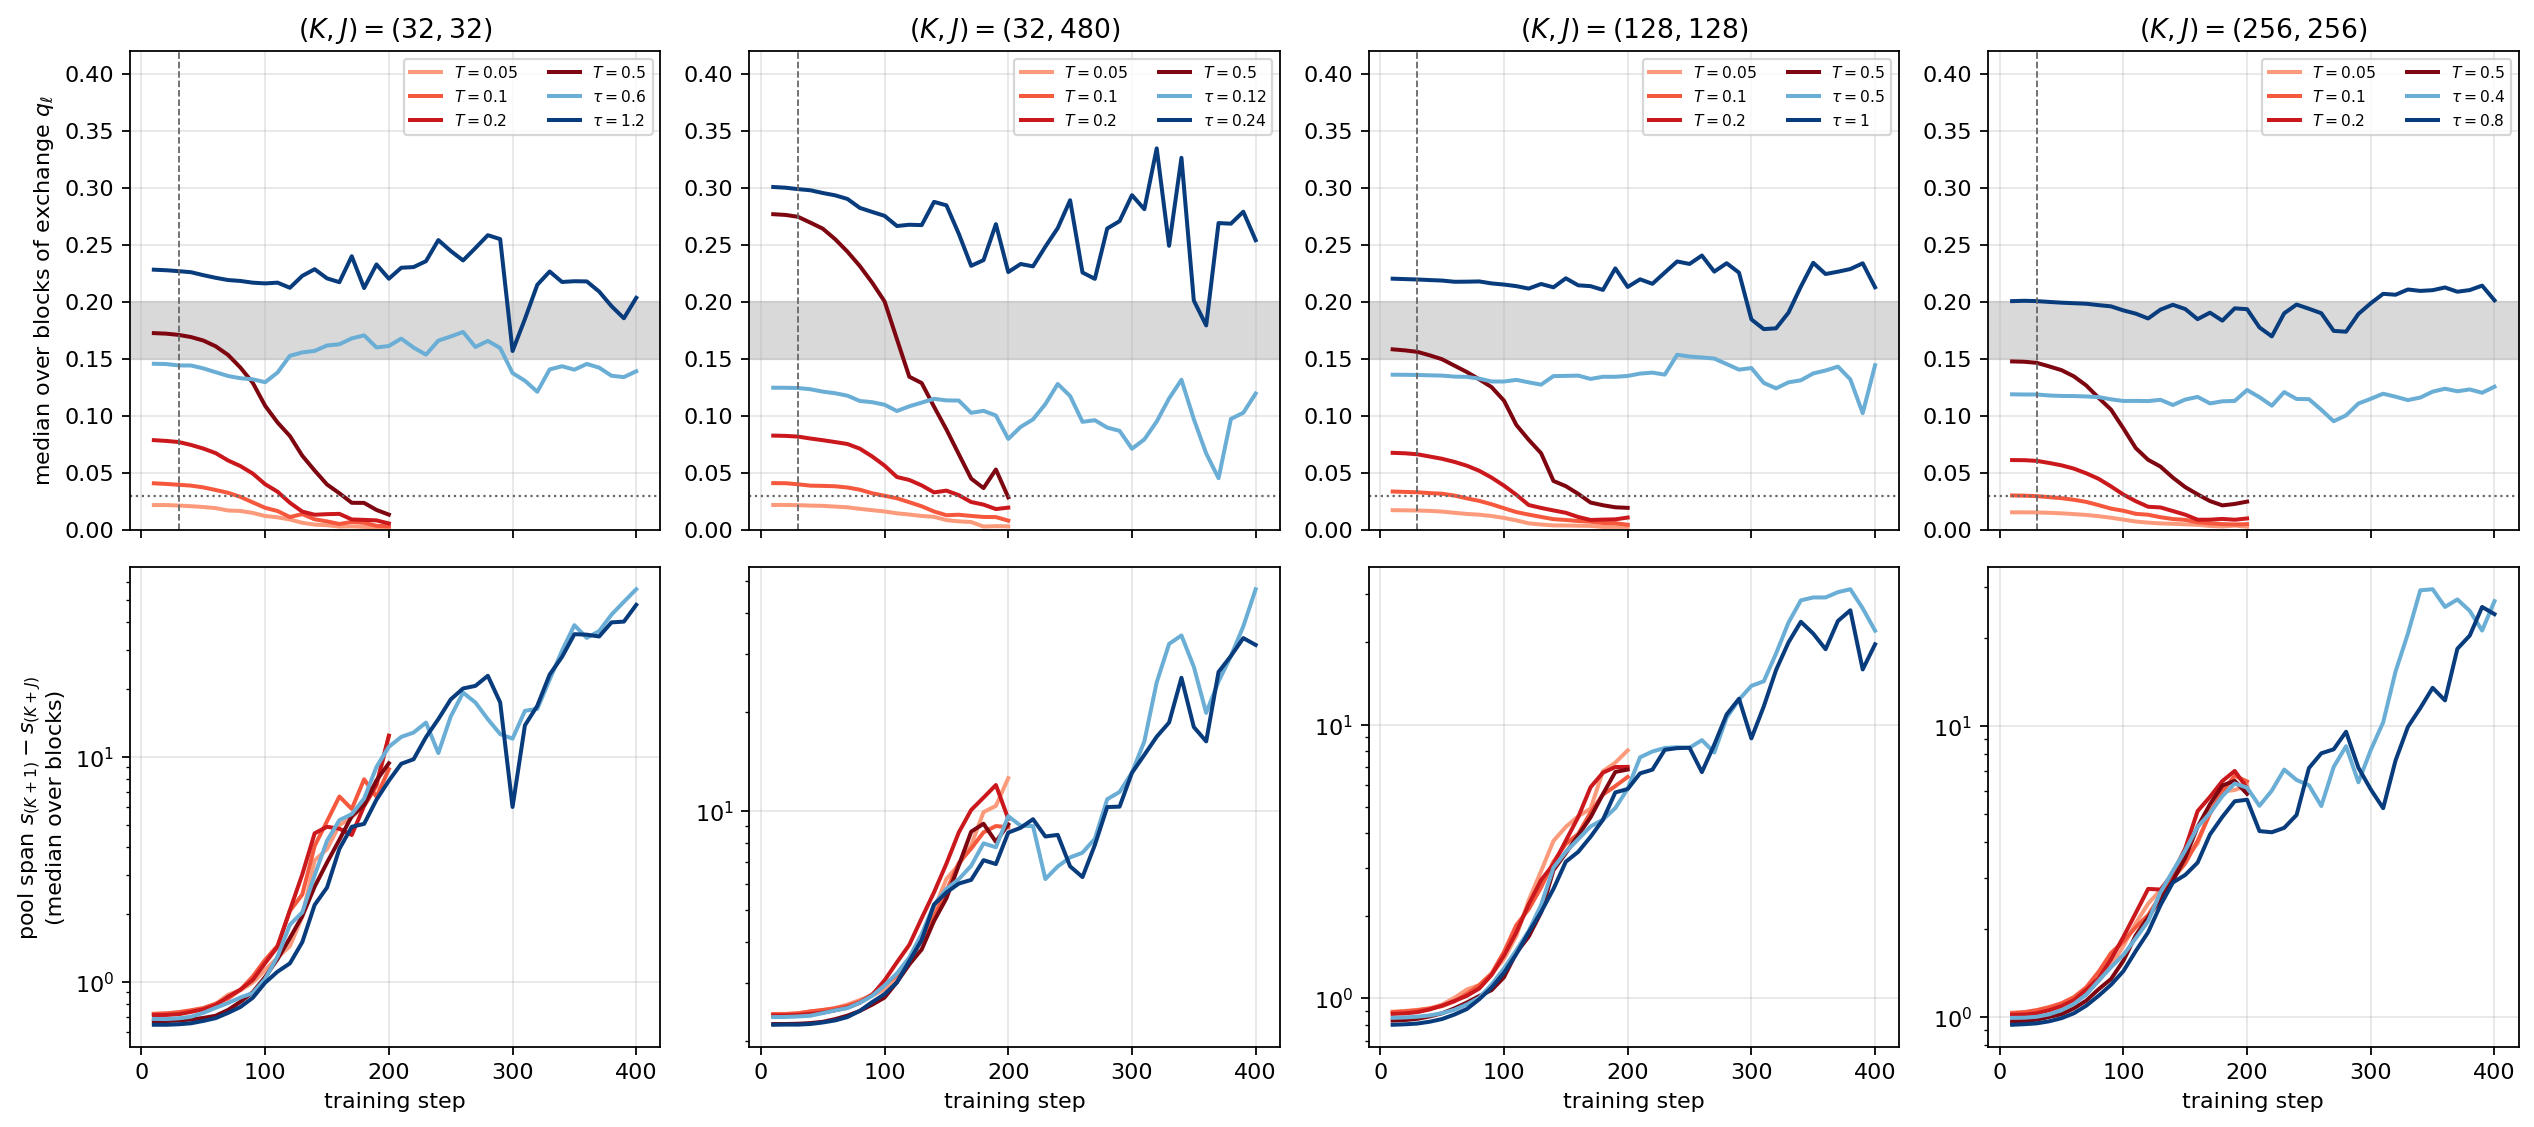
\includegraphics[width=\textwidth]{figures/policy-cr/pc_calib.png}
\caption{Calibration probes, one column per cell. Top: median over blocks of
the exchange $q_\ell$ against step for the absolute widths (reds, $T = 0.05$ to
$0.5$) and the span-relative widths (blues); grey band the target $[0.15,
0.20]$, dotted line $3\%$, dashed line step 30. Bottom: the pool span (median over
blocks, log scale): the same growth in every probe.}
\label{fig:calib}
\end{figure}

% ============================================================
\section{The failure}
% ============================================================

The eight runs (constant and annealed $\tau$, four cells) were launched with
the likelihood-ratio estimator, $\gamma = 1$ and the calibrated span-relative
widths, and stopped at steps 2540--2800 when it was clear they did not learn:

\begin{center}\small
\begin{tabular}{lccccc}
\toprule
clean validation CE & step 500 & 1000 & 1500 & 2000 & 2500 \\
\midrule
$(32,32)$ constant / annealed   & 6.90 / 6.65 & 6.25 / 6.10 & 5.96 / 6.00 & 5.97 / 5.96 & 5.95 / 6.00 \\
$(32,480)$ constant / annealed  & 7.11 / 7.20 & 6.48 / 6.35 & 6.27 / 6.15 & 6.08 / 6.15 & 6.09 / 6.02 \\
$(128,128)$ constant / annealed & 11.51 / 6.96 & 6.46 / 6.47 & 6.09 / 6.03 & 6.04 / 5.97 & 6.03 / 5.99 \\
$(256,256)$ constant / annealed & 7.54 / 7.22 & 6.39 / 6.36 & 6.14 / 6.03 & 6.05 / 5.99 & 5.98 / 5.96 \\
\midrule
RBLapSum $T=2$, $(32,480)$       & 2.69 & 2.23 & 2.04 & 1.95 & 1.89 \\
\bottomrule
\end{tabular}
\end{center}

Every run settles at $5.95$--$6.09$, the unigram level of this data (the level
the collapsed post-norm cells of the code-residual note reached). The gradient
norm before clipping was $10^3$--$10^5$ on every logged step (Figure~\ref{fig:gn});
with \code{grad\_clip = 1} every step was clipped. The advantage $c_b - B$ had
mean $-0.4$ to $-1.5$ at step 500: the EMA baseline lags the falling CE. The
constant and annealed member of each pair compute the same thing until step
1000, yet differ by $0.09$--$0.32$ at step 500 ($4.5$ where one run was in a
loss spike): the run-to-run spread of one configuration under this estimator.

\begin{figure}[htb]\centering
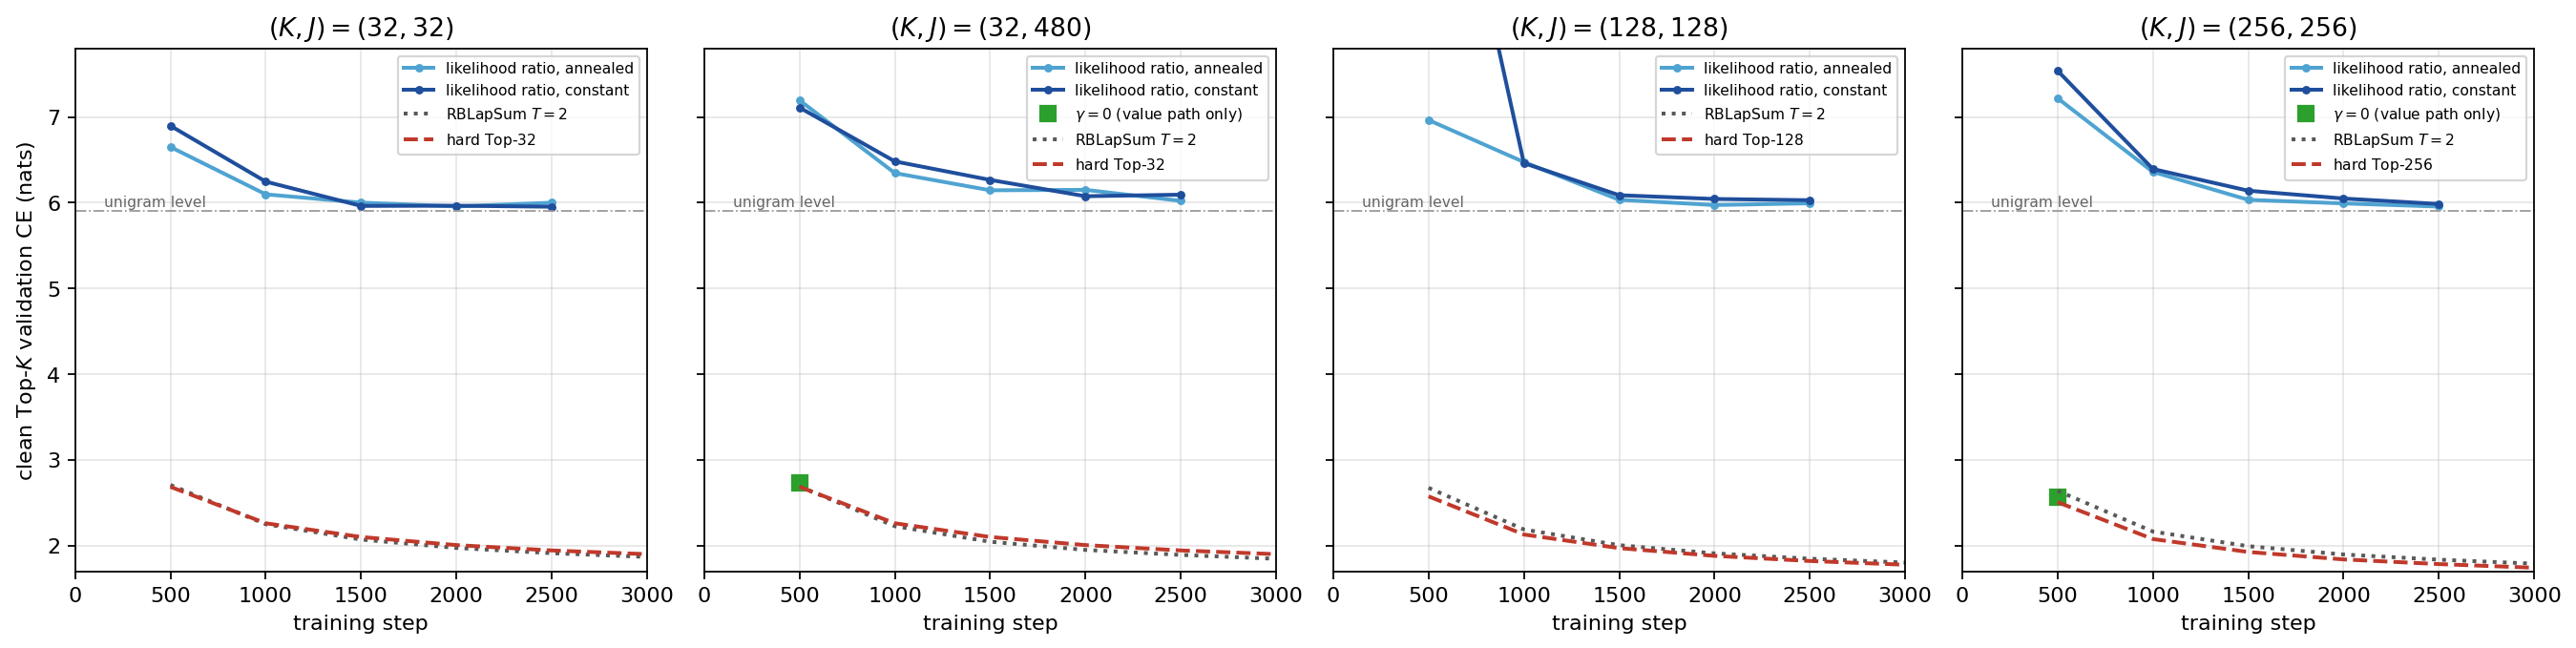
\includegraphics[width=\textwidth]{figures/policy-cr/pf_failure.png}
\caption{Clean validation CE of the eight likelihood-ratio runs (blue: constant,
light blue: annealed width) against RBLapSum $T=2$ (dotted) and hard Top-$K$
(dashed red), first 3000 steps; green squares: the $\gamma = 0$ controls at step
500. Dash-dot line: the unigram level.}
\label{fig:fail}
\end{figure}

% ============================================================
\section{Diagnosis}
\label{sec:diag}
% ============================================================

\subsection*{Anatomy of the estimator}

In \eqref{eq:lr} every pool member of every gate instance contributes
$\pm 1/T$ times the sequence's advantage, whether or not its noise changed the
support: a member far inside or far outside the support contributes a term of
the same size as one at the boundary. The expectation of those terms is zero;
each sample is not. For one sequence there are $8 \times 512 \times (K{+}J)$
such terms -- $2.1 \times 10^6$ at $K{+}J = 512$ -- and one scalar
$c_b - B$ multiplies all of them, including the effect of an action at
position $t$ on the losses of earlier positions, which it cannot influence.
The signal is the covariance between the CE and the rare noise configurations
that move a member across the $K$-th noisy score, so it comes from the members
within about $T$ of their threshold, while the variance grows with all
$L\,T_{\mathrm{seq}}\,(K{+}J)$ coordinates; a scalar baseline removes only the
part of $c_b$ common to all sequences.

\subsection*{Measurement on a fixed batch}

\code{scripts/policy\_grad\_probe.py} fixes one checkpoint and one training
micro-batch ($24 \times 512$ tokens) of the $(32, 480)$ cell and draws the
noise $M = 64$ times. For each estimator it reports the norm of the Monte Carlo
mean, the per-draw noise $\sqrt{\operatorname{tr}\widehat\Sigma}$, the
bias-corrected signal $|\mathbb E\,\hat g| = (\|\bar g\|^2 -
\operatorname{tr}\widehat\Sigma / M)^{1/2}$ and the cosine of the mean with
$g_{\mathrm{value}}$, per layer and for the whole model. Three states: the
initialization, the likelihood-ratio run's own checkpoint at step 2000, and the
RBLapSum $T=2$ run at step 2000 loaded into the policy model.

\begin{center}\small
\begin{tabular}{lccccccc}
\toprule
state (clean CE) & $\|g_{\mathrm{value}}\|$ & \multicolumn{2}{c}{likelihood ratio} &
\multicolumn{2}{c}{RB, full scope} & \multicolumn{2}{c}{RB, first order} \\
 & & noise & SNR & noise & SNR & noise & SNR \\
\midrule
initialization (11.34)        & 1.13  & $3.7 \times 10^4$ & $0.009$ & 240  & $0.013$ & 0.95  & 0.60 \\
likelihood-ratio run, 2000 (6.03) & 0.91  & $6.7 \times 10^3$ & $0.10$  & 0.60 & $0.20$  & 0.063 & 1.1 \\
RBLapSum run, 2000 (1.82)     & 0.35  & $2.1 \times 10^4$ & $\approx 0$ & 5.1  & $0.08$  & 0.25  & 0.88 \\
\bottomrule
\end{tabular}
\end{center}

SNR is the per-draw ratio $|\mathbb E\,\hat g| / \sqrt{\operatorname{tr}\Sigma}$.
The likelihood-ratio noise is $10^4$--$10^5$ times the value gradient; at the
initialization and at the RBLapSum state its 64-draw mean is explained by the
noise alone. The ratio $\gamma_* = \|g_{\mathrm{value}}\| /
\operatorname{median}_m \|\hat g_{\mathrm{LR}}^{(m)}\|$ is $3.0 \times 10^{-5}$,
$1.5 \times 10^{-4}$ and $1.7 \times 10^{-5}$ at the three states. The per-layer
picture (Figure~\ref{fig:probe}) is the same in every block: the noise
reaches every parameter group upstream of a gate, including the embedding. The
full-scope Rao--Blackwell noise (Section~\ref{sec:rb}) is largest in the first
blocks, which receive the products of every later gate's selection term.

\begin{figure}[htb]\centering
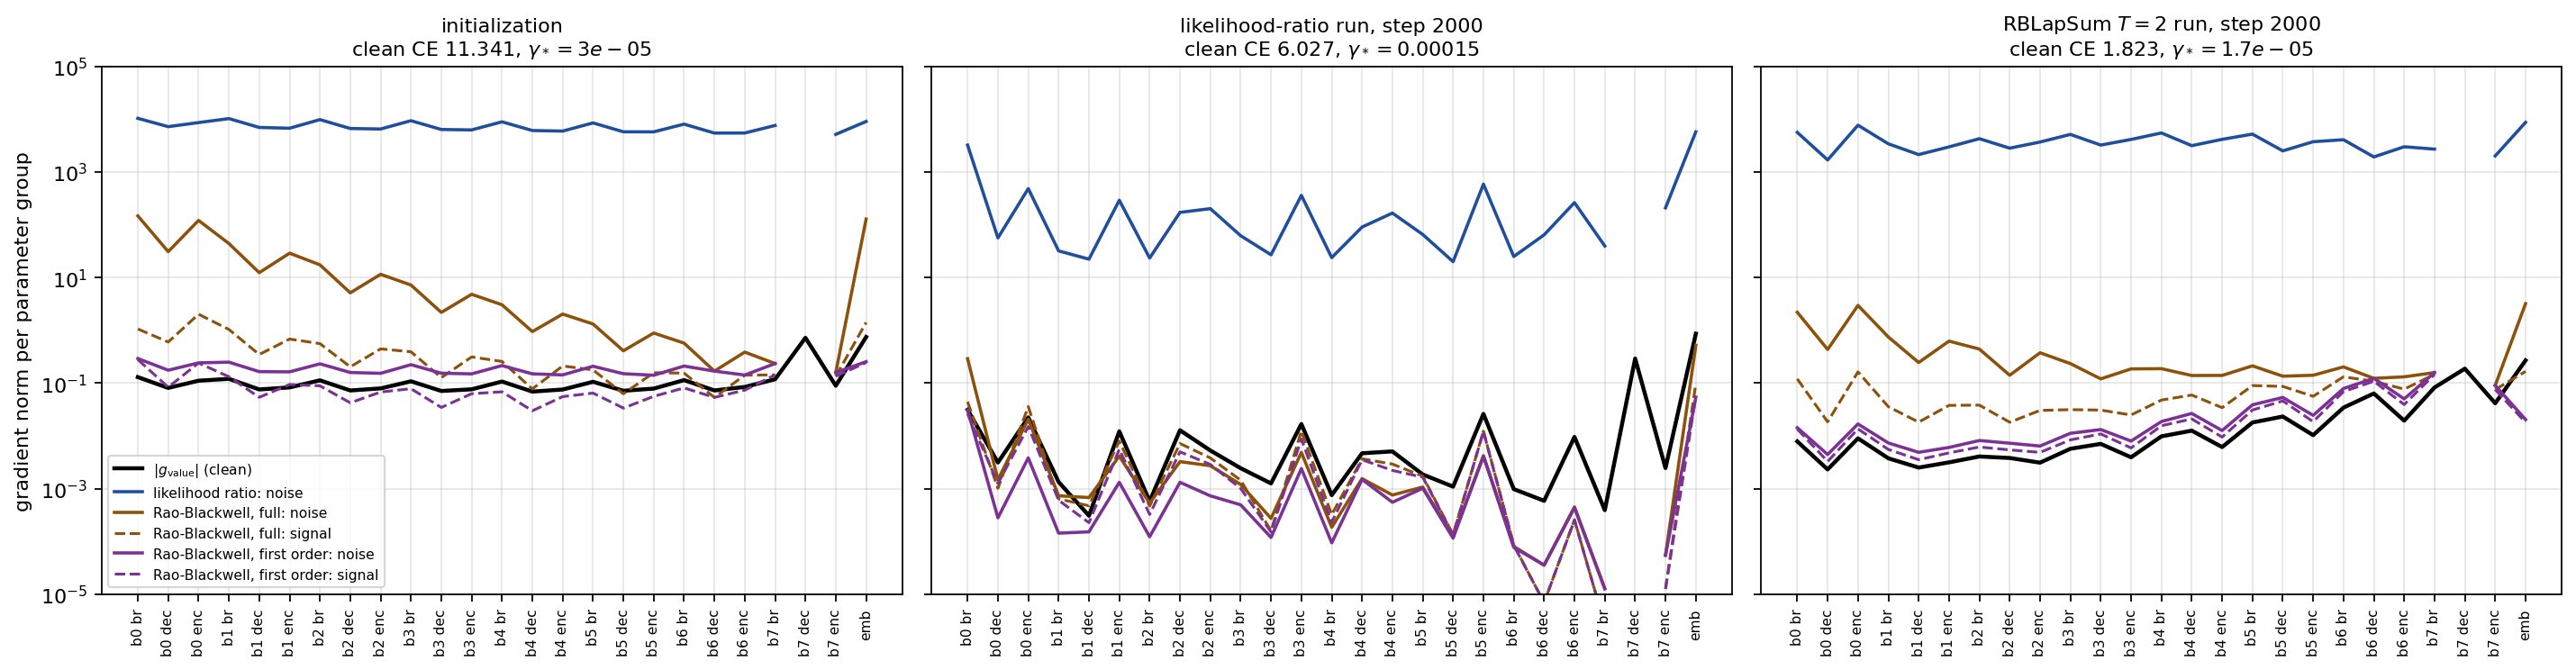
\includegraphics[width=\textwidth]{figures/policy-cr/pf_probe.png}
\caption{Per parameter group (block branches, encoder, decoder; embedding last)
at the three probed states: $\|g_{\mathrm{value}}\|$ (black) and the per-draw
noise (solid) of the likelihood-ratio estimator (blue), the Rao--Blackwell
estimator with the full scope (brown) and with the first-order scope (purple);
dashed, the bias-corrected signal of the two Rao--Blackwell estimators (the
likelihood-ratio mean is not resolved by 64 draws). Log scale. The last block's
decoder receives no selection gradient.}
\label{fig:probe}
\end{figure}

\subsection*{Clipping}

With $\|\hat g\| = 10^3$--$10^5$ and clipping at 1, the combined gradient is
scaled by $10^{-3}$--$10^{-5}$ on every step, so the value-gradient part of the
update is scaled by the same factor while its direction is set by the noise.
Under Adam's per-element normalization the same holds element by element: the
second-moment estimate is set by the noise, and the value signal moves each
parameter by a fraction of order $\|g_{\mathrm{value}}\| / \|\hat g\|$ of its
step. The update is a unit-norm, mostly random step with a small hard-path
component -- consistent with the unigram plateau, and with the spread between
the two members of a pair that compute the same thing until step 1000.

\subsection*{Controls}

\paragraph{$\gamma = 0$.} The same forward -- sampled supports at the calibrated
exchange -- with the selection term removed (\code{policy\_support\_scale: 0})
trains like the references: clean validation CE at step 500 is $2.732$ at
$(32, 480)$ (RBLapSum $2.689$, hard Top-32 $2.685$) and $2.569$ at $(256, 256)$
(RBLapSum $2.639$, hard Top-256 $2.506$), with gradient norms $0.26$--$0.28$.
The sampled forward itself costs about $0.04$ at step 500 at $(32, 480)$; the
loss of the campaign runs is the selection term's.

\paragraph{A smaller $\gamma$.} Scaling the likelihood-ratio term down to the
size of the value gradient trades the noise for nothing: with $\gamma_* = 3.05
\times 10^{-5}$ from the initialization probe, four runs of 600 steps scale it
by $\gamma \in \{0, 0.1\gamma_*, \gamma_*, 10\gamma_*\}$. They ran beside the
main run with micro-batches of 8 (the same 96 sequences per step) and therefore
validate on the first 320 of the usual 960 windows: their validation CE is
comparable among themselves, not with the other tables.

\begin{center}\small
\begin{tabular}{lcccc}
\toprule
$\gamma$ & $0$ & $0.1\gamma_*$ & $\gamma_*$ & $10\gamma_*$ \\
\midrule
validation CE, step 500 (320 windows) & 2.638 & 2.802 & 3.424 & 4.555 \\
noise-off training CE, step 400 & 2.904 & 3.111 & 3.832 & 4.901 \\
gradient norm, step 100 & 0.53 & 0.63 & 2.78 & 20.3 \\
\bottomrule
\end{tabular}
\end{center}

The loss rises monotonically with $\gamma$ from $\gamma = 0$ on
(Figure~\ref{fig:salvage}): no scale of the term makes it useful. Even $0.1\gamma_*$, at which the term's whole-model noise
is about a tenth of the value gradient, costs $0.16$ at step 500. A plausible
reason, not measured here: under per-element normalization what matters is the
noise of each parameter, and the term's noise is concentrated in the parameters
it reaches most directly (the encoders), where it dominates the update even at a
small global share.

\begin{figure}[htb]\centering
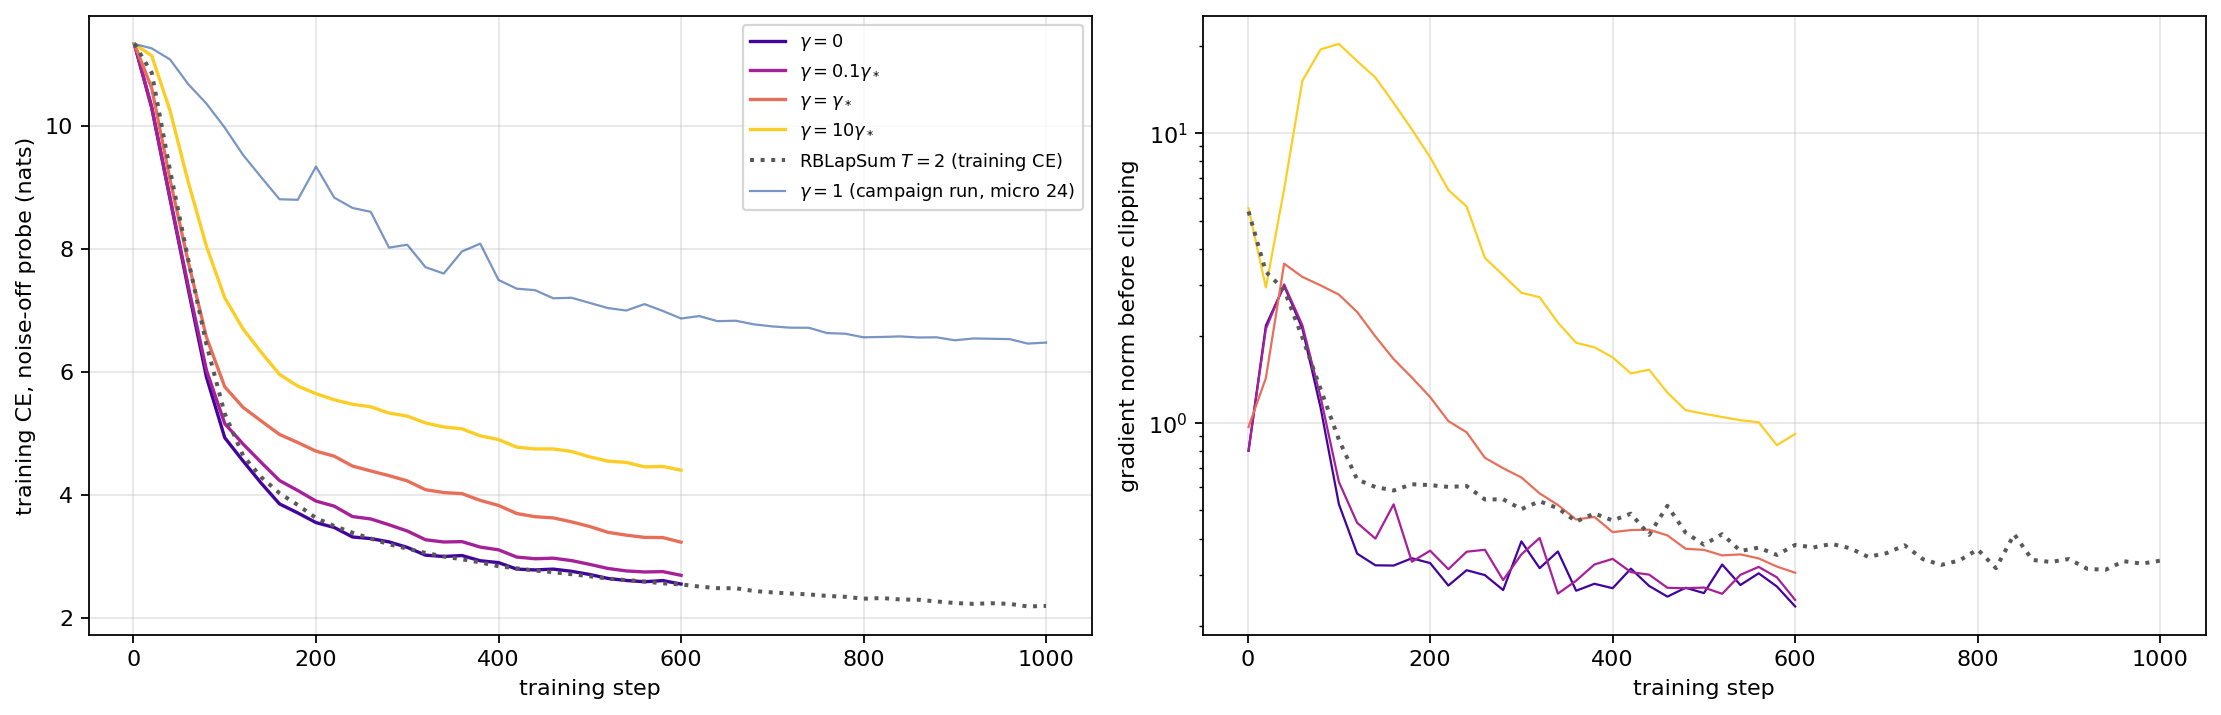
\includegraphics[width=\textwidth]{figures/policy-cr/pf_salvage.png}
\caption{The $\gamma$ grid at $(32, 480)$, 600 steps: noise-off training CE
(left) and gradient norm before clipping (right) for $\gamma = 0$,
$0.1\gamma_*$, $\gamma_*$, $10\gamma_*$ ($\gamma_* = 3.05 \times 10^{-5}$),
with RBLapSum $T = 2$ (dotted, its training CE) and the $\gamma = 1$ campaign run
(blue).}
\label{fig:salvage}
\end{figure}

\subsection*{Realized swap differences are discontinuous}

An estimator built on realized loss differences -- the likelihood ratio, or an
exact version of the conditional estimator below -- needs $L(i \text{ in}) -
L(i \text{ out})$ for a single swap. \code{scripts/policy\_swap\_probe.py}
measures it on the RBLapSum state: on a fixed noise draw of the earlier gates
and the probed gate, a forward hook applies one swap at one token, the later
gates' noise is redrawn 16 times, and the summed token CE of $2 \times 512$
tokens is compared with the unswapped forward (fp32; the forward is
deterministic). Over 72 (gate, token, member) triples near the threshold at
gates 0, 3 and 7, the per-draw standard deviation of the exact difference has
median $4.9$ nats, its 16-draw mean is not resolved (median standard error
$1.2$), and the first-order difference $g_i v_i - g_j v_j$ has median magnitude
$0.001$. One swap moves the input of every later gate at that token, and
through attention the later tokens, so later supports flip at near-ties; each
flip changes a token's loss by a finite amount. Realized loss differences are
dominated by these re-selections, not by the swap's own effect.

% ============================================================
\section{The Rao--Blackwellized estimator}
\label{sec:rb}
% ============================================================

\paragraph{Derivation.}
Fix one pool member $i$ and all noise except its own. Member $i$ is selected iff
$u_i + \varepsilon_i > \theta_i$, where $\theta_i$ is the $K$-th largest noisy
score among the other members: $r_{(K+1)}$ if $i$ is selected, $r_{(K)}$ if not;
let $j$ be its owner, the member $i$ swaps with. For $\varepsilon \sim
\mathrm{Laplace}(0, T)$, $\mathbb E[\sgn(\varepsilon)\,\mathbf 1\{\varepsilon >
c\}] = \tfrac12 e^{-|c|/T} = T\,p_T(c)$ with $p_T(x) = e^{-|x|/T} / (2T)$, so
the conditional expectation of the likelihood-ratio sample over the member's
own noise is
\begin{equation}
\mathbb E\!\left[(L - B)\,\frac{\sgn(\varepsilon_i)}{T} \,\middle|\, \varepsilon_{-i}\right]
= p_T(\theta_i - u_i)\,\big(L(i \text{ in}, j \text{ out}) - L(i \text{ out}, j \text{ in})\big).
\label{eq:rb}
\end{equation}
The baseline drops out; members far from their threshold contribute
$\sim e^{-|\theta_i - u_i|/T}$ instead of $\pm 1/T$; by the law of total variance
the estimator has no more variance than \eqref{eq:lr} per coordinate. The
single-swap difference is taken to first order from the backpropagated gradient
$g = \partial L / \partial y$ at the sampled support,
\begin{equation}
\hat g_{\mathrm{RB}, i} = \gamma\, p_T(\theta_i - u_i)\,\big(g_i v_i - g_j v_j\big),
\label{eq:rblin}
\end{equation}
with the value path unchanged ($\partial L / \partial v_i = g_i m_i$). For a
loss linear in the gate output the first-order difference is exact, and a Monte
Carlo test confirms that \eqref{eq:rblin} and \eqref{eq:lr} then agree in
expectation for every pool member, in the absolute and the relative widths
(\code{tests/test\_policy\_rao\_blackwell.py}). It is
\code{policy\_estimator: rao\_blackwell}
(\code{wsparse.bottleneck.laplace\_policy.RaoBlackwellSelect}).

\paragraph{Scope along the carry.}
With the total incoming $g$ in \eqref{eq:rblin} (\code{policy\_rb\_scope: full}),
the gradient of a boundary member picks up a factor $m_i + \gamma\, p_T |v_i|$ at
every gate it passes, and along the identity carry of the code residual those
factors multiply -- the mechanism that collapsed pool-scope RBLapSum at depth.
The two full-scope runs reached gradient norms of $4.9 \times 10^3$--$1.1 \times
10^4$ at $(32, 480)$ and $1.1 \times 10^5$--$8.5 \times 10^5$ at $(256, 256)$
within 120 steps (Figure~\ref{fig:gn}). \code{policy\_rb\_scope: first\_order}
linearizes the swap with the gradient that reached the gate along hard paths (a
second backward pass): the first-order term of the swap at fixed later
selections, which is also the term that does not inherit the later re-selections
of the previous paragraph. In the probe its noise is $0.06$--$0.95$, of the
order of $\|g_{\mathrm{value}}\|$, with signal-to-noise $0.6$--$1.1$ per draw.

\paragraph{Width gradient.}
A relative width makes the sampled support invariant to a common shift
\emph{and} a common rescaling of the pool scores, so the exact selection
gradient satisfies $\langle \nabla_s \mathcal J, \mathbf 1 \rangle = 0$ and
$\langle \nabla_s \mathcal J, s \rangle = 0$ (Euler's identity for a function
homogeneous of degree 0). The original implementation detaches the width (the
``frozen-scale'' partial gradient), whose component along $s$ pushes the scale
the width then follows. Three treatments were run at $(32, 480)$ with the
first-order scope:

\begin{center}\small
\begin{tabular}{lccccc}
\toprule
width gradient & \multicolumn{2}{c}{probe} & pool span & \multicolumn{2}{c}{clean CE} \\
 & noise & signal & step 100 $\to$ 500 & step 500 & step 1000 \\
\midrule
\code{frozen} (detached width)      & 0.44 & 0.37 & $13 \to 2.2\times10^5$ & 5.30 & -- \\
\code{through} (span differentiated) & 1.29 & 0.37 & $3.1 \to 3.1$ & 2.97 & 2.56 \\
\code{project} (radial part removed) & 0.40 & 0.37 & $4.3 \to 2.6$ & 2.78 & \PH{P1000} \\
\bottomrule
\end{tabular}
\end{center}

(Probe at the RBLapSum state with micro-batches of 8, $\|g_{\mathrm{value}}\| =
0.58$, value-path noise $0.22$; the three means agree, cosine $0.91$ between
\code{frozen} and \code{through}.) The frozen gradient, followed by a low-noise
estimator, drives the pool span up exponentially -- the runaway the tsweep note
recorded for RBLapSum's relative widths. Differentiating through the span
removes the push but routes the correction through the two order statistics
$s_{(K+1)}$ and $s_{(K+J)}$, which triples the per-draw noise. The third
treatment keeps the frozen gradient $g$ of the selection path and removes its
component along the centred scores,
\begin{equation}
\tilde g = g - \frac{\langle g, u \rangle}{\langle u, u \rangle}\,u,
\label{eq:project}
\end{equation}
the minimum-norm correction that restores both identities
(\code{policy\_width\_gradient: project}); its noise is the lowest of the three.
It is not the exact gradient. By Euler's identity the exact one removes the same
radial amount $\langle g, s \rangle$ but places it on the two scores that define
the span, $-\langle g, s\rangle\,(e_{(K+1)} - e_{(K+J)}) / (s_{(K+1)} - s_{(K+J)})$;
the two differ by a vector orthogonal to $s$ whose size is set by the radial
component of the frozen gradient.
Averaging \eqref{eq:rblin} over further pool-noise draws in the backward
(\code{policy\_rb\_samples}) halves the noise of \code{through} ($0.62$ at 8
draws) and leaves the frozen variant's unchanged ($0.43$): the remaining noise
is in $g$, not in the sampled thresholds.

% ============================================================
\section{Results}
\label{sec:results}
% ============================================================

\subsection*{The repaired estimator at $(32, 480)$}

One run of 20k steps at $(32, 480)$ with the three changes --
\code{policy\_estimator: rao\_blackwell}, \code{policy\_rb\_scope: first\_order},
\code{policy\_width\_gradient: project} -- and everything else as in the
campaign: the span-relative width at the calibrated $\tau_0 = 0.16$, constant,
$\gamma = 1$ (run \code{zu\_rbfo\_proj\_k32\_j480\_t0p16\_const}, config in
\code{configs/policy\_cr/}). Clean validation CE, with the
differences $\Delta_{\mathrm{P-RB}} = L^{\mathrm{policy}} - L^{\mathrm{RBLapSum}}$
and $\Delta_{\mathrm{P-hard}} = L^{\mathrm{policy}} - L^{\mathrm{hard\ Top\text{-}32}}$
(negative: the policy is better):

%%RESULT_TABLE%%

%%RESULT_TEXT%%

\begin{figure}[htb]\centering
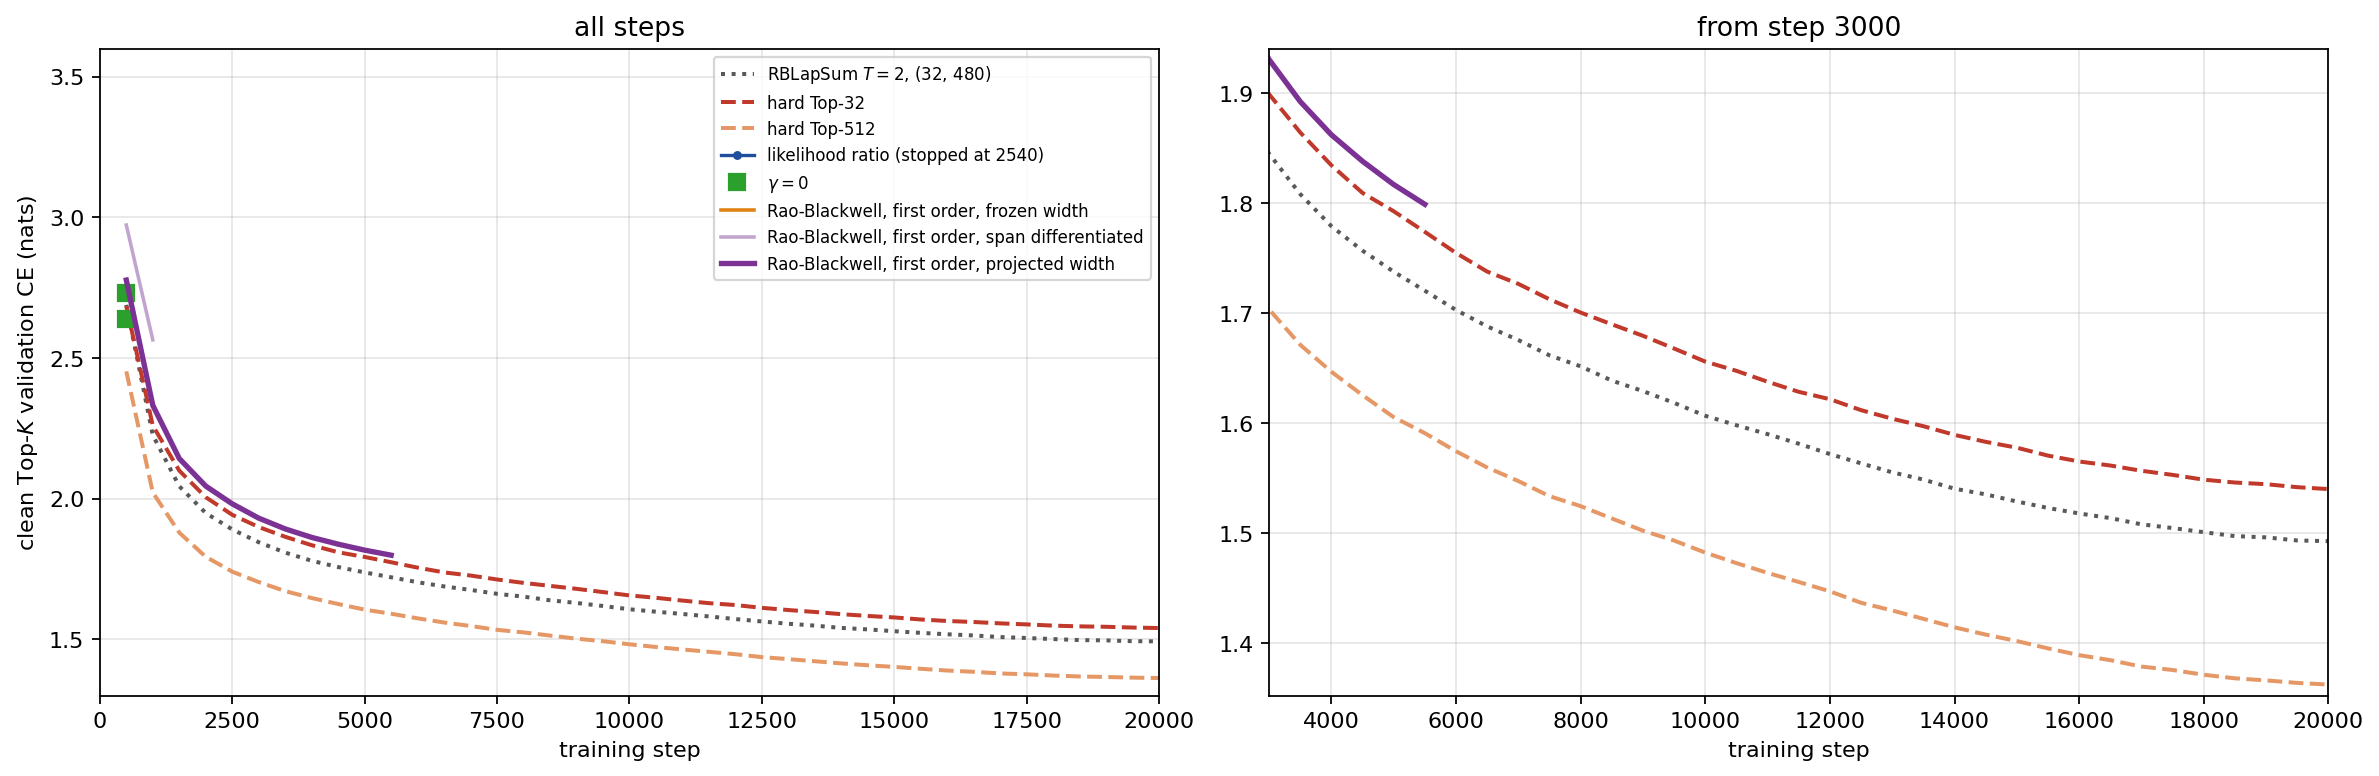
\includegraphics[width=\textwidth]{figures/policy-cr/pf_fix.png}
\caption{Clean validation CE at $(32, 480)$: the repaired estimator (projected
width, dark purple) against RBLapSum $T = 2$ (dotted), hard Top-32 and Top-512
(dashed), the two other width gradients with the first-order scope (span
differentiated, light purple, stopped at step 1060; frozen, orange, stopped at
step 700 after the span runaway), the likelihood-ratio campaign run (blue,
stopped at 2540) and $\gamma = 0$ (green). Right: from step 3000 on a tight scale.}
\label{fig:fix}
\end{figure}

\begin{figure}[htb]\centering
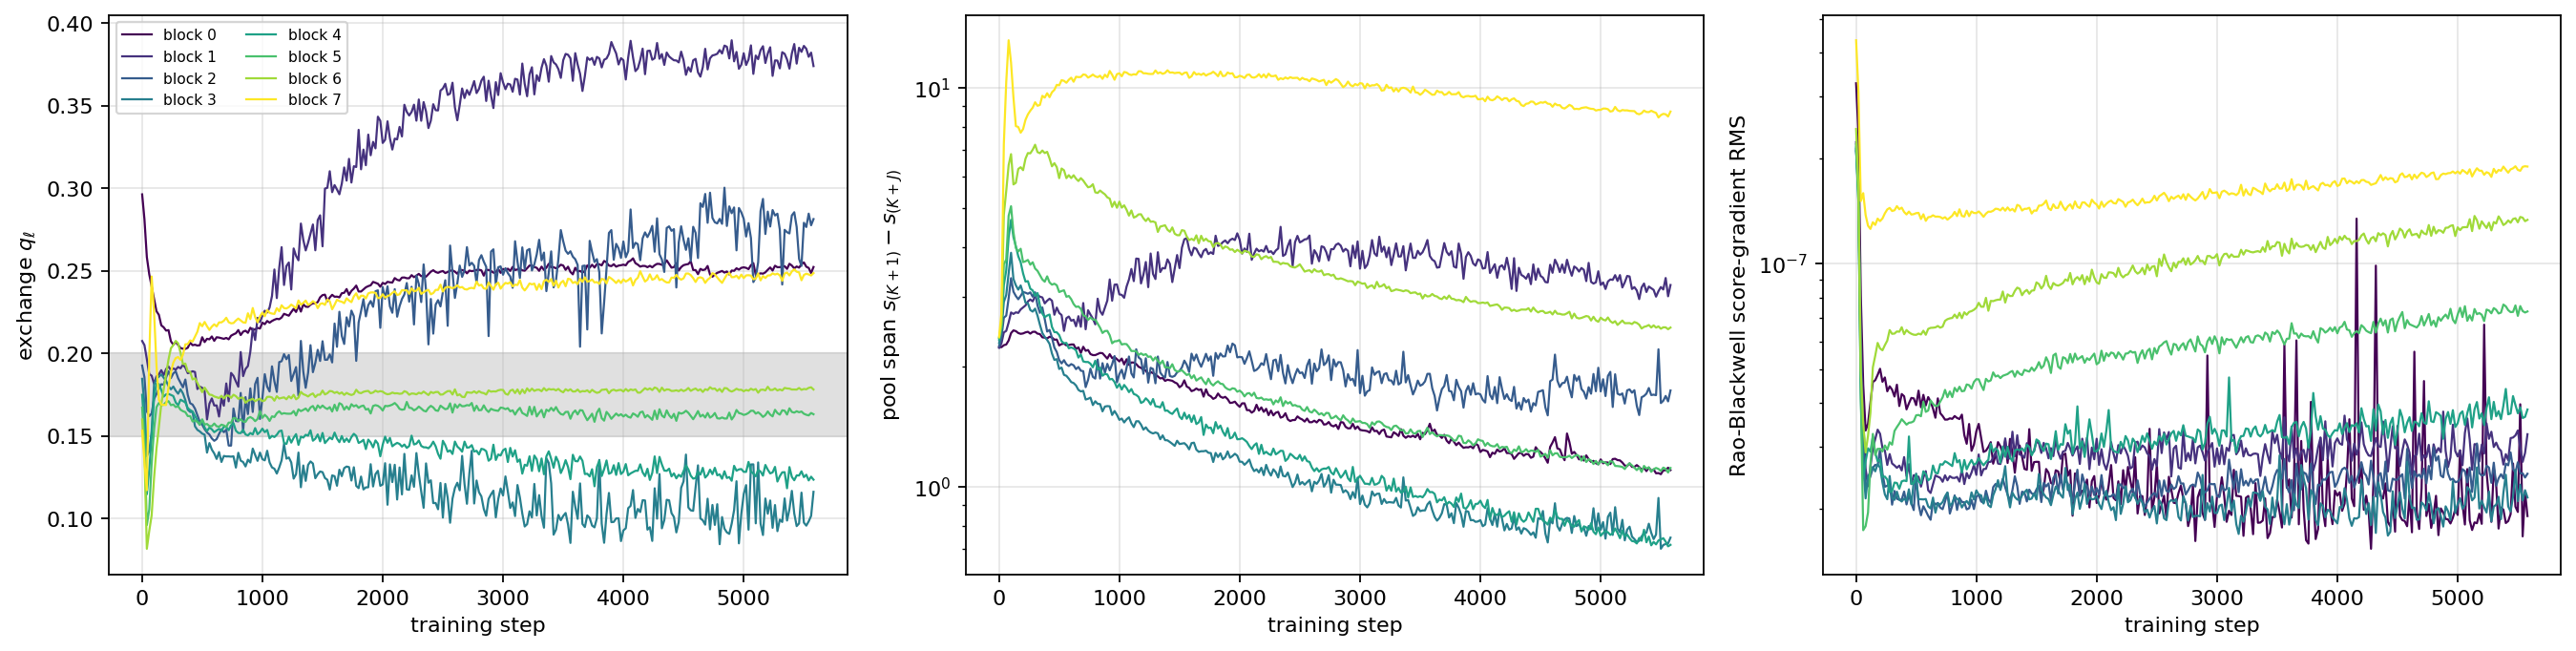
\includegraphics[width=\textwidth]{figures/policy-cr/pf_rb_blocks.png}
\caption{The repaired run, per block (colour from block 0, dark, to block 7,
light): exchange fraction $q_\ell$ (grey band the calibration target), pool span
(log), and the RMS of the Rao--Blackwell score gradient (log).}
\label{fig:rbblocks}
\end{figure}

\begin{figure}[htb]\centering
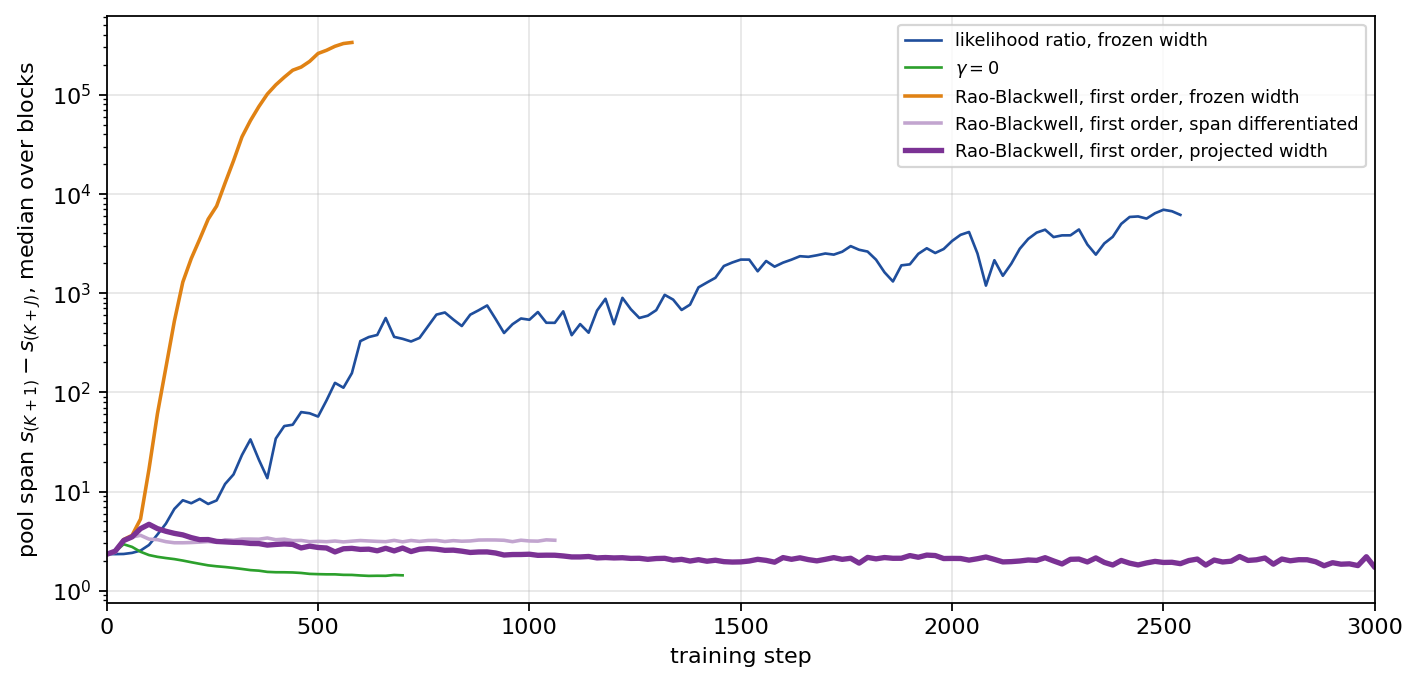
\includegraphics[width=.75\textwidth]{figures/policy-cr/pf_span.png}
\caption{Pool span (median over blocks) against step at $(32, 480)$: the
likelihood-ratio run and the frozen-width Rao--Blackwell run grow it without
bound, the scale-free variants (span differentiated, projected) and $\gamma = 0$
do not.}
\label{fig:span}
\end{figure}

\subsection*{A second cell: $(256, 256)$}

The same three changes at $(256, 256)$, with the cell's calibrated
$\tau_0 = 0.67$, ran for 1500 steps of the 20k schedule beside the main run (micro-batches of 8 with
120 validation batches: the same 960 windows as every other table); the run is
\code{zu\_rbfo\_proj\_k256\_j256\_t0p67\_const}. This is the cell where the
full scope reached gradient norms of $8.5 \times 10^5$.

\begin{center}\small
\begin{tabular}{lccc}
\toprule
clean validation CE & step 500 & 1000 & 1500 \\
\midrule
policy, repaired          & 2.620 & 2.165 & 2.010 \\
RBLapSum $T = 2$          & 2.639 & 2.163 & 1.992 \\
hard Top-256              & 2.506 & 2.076 & 1.925 \\
hard Top-512              & 2.453 & 2.022 & 1.879 \\
$\gamma = 0$ (vienna)     & 2.569 & --    & -- \\
\bottomrule
\end{tabular}
\end{center}

Over the first 1500 steps the repaired estimator is level with RBLapSum --
$-0.019$, $+0.002$, $+0.018$ at steps 500, 1000, 1500 -- and $0.085$--$0.114$
above hard Top-256, the order the code-residual note found for this cell at 20k
(RBLapSum $0.034$ above hard Top-256). The run is stable where the full scope
diverged: gradient norm median $0.60$ after step 500 (4 of 50 logged steps above
the clip), block-averaged exchange $0.175$--$0.184$, pool span $0.84$--$1.05$,
self-gain $\gamma\,p\,|v|$ of the member nearest the threshold about $2.2$ (median
over blocks). With 1500 of 20k steps this is a check that the repair carries
over to a large $K$, not a comparison of final losses.


% ============================================================
\section{Interpretation}
% ============================================================

Four properties of this setting -- none of them a property of the expected
sampled CE as an objective -- stopped the original method, and each change
addresses one.

\emph{Credit assignment.} The likelihood-ratio estimator assigns one scalar
outcome to about $2 \times 10^6$ independent noise coordinates per sequence and
lets each of them contribute $\pm 1/T$; whether a coordinate moved the support is
left to cancellation across samples that one update never sees. The measured
noise is $10^4$--$10^5$ times the value gradient, so no reweighting of the term
($\gamma$, a better scalar baseline, reward-to-go) can make one sample
informative: it can only make the term small. Conditioning on all other noise
replaces each coordinate's $\pm 1/T$ by the probability density that its own
noise crosses its threshold, which is what makes the sum informative, and the
remaining factor is a single swap's loss difference.

\emph{Discontinuity of the realized loss.} That swap difference, realized on the
network, is dominated by the re-selections it triggers at later gates and later
tokens (per-draw spread about $5$ nats against a first-order effect of $10^{-3}$).
Any estimator that waits for realized loss differences inherits that spread.
The first-order difference from the backpropagated gradient is the part that
does not depend on later flips, and it is what RBLapSum also uses, through a
deterministic kernel instead of a sampled threshold.

\emph{The carry.} Along the identity carry of the code residual, a selection
term computed from the total downstream gradient multiplies with the next gate's
own; with the narrow widths needed for a moderate exchange the factor per gate
is several units, and the full scope diverged within 100 steps. The first-order
scope is the same restriction the code-residual note found necessary for
RBLapSum at depth.

\emph{The width's symmetry.} A width proportional to the scores makes the
selection invariant to their scale, but the detached-width gradient still
pushes the scale. With the likelihood-ratio estimator this push was diluted by
noise and appeared as a slow growth of the span; with the low-noise estimator
it became an exponential runaway. Projecting the push out restores the
symmetry the exact gradient has, and it removes rather than adds variance.

%%INTERP_RESULT%%

% ============================================================
\section{Scope}
% ============================================================

The repaired estimator was trained to completion on one cell, $(32, 480)$, with
one seed and the constant width; the other three cells and the annealed width --
the campaign's original question -- were not rerun with it, so the comparison of
constant and annealed widths remains open. The $\gamma = 0$ controls ran to step
700 (vienna) and 600 (zurich, as part of the $\gamma$ grid), not to 20k, so the
net value of the selection term late in training is measured against RBLapSum
and hard Top-$K$, not against the same sampled forward without it. The probes use
one checkpoint, one cell and one micro-batch (24 sequences; 8 for the
width-variant probe); their per-draw signal-to-noise ratios refer to that batch
size, and a training step averages four such micro-batches. The span-relative
width was calibrated at step 30 by the plan's rule; its exchange during the
repaired run is reported, not re-tuned. The first-order Rao--Blackwell estimator
is unbiased only for losses linear in the gate output; for the network its bias
is the omitted re-selection effects, which the swap probe shows to be
unresolvable by direct sampling at this scale. The reference runs were trained
on another box of the same card model (bf16, not bit-reproducible across
machines), and the hard baselines carry the output norm while the policy and
RBLapSum runs do not.

\begin{figure}[htb]\centering
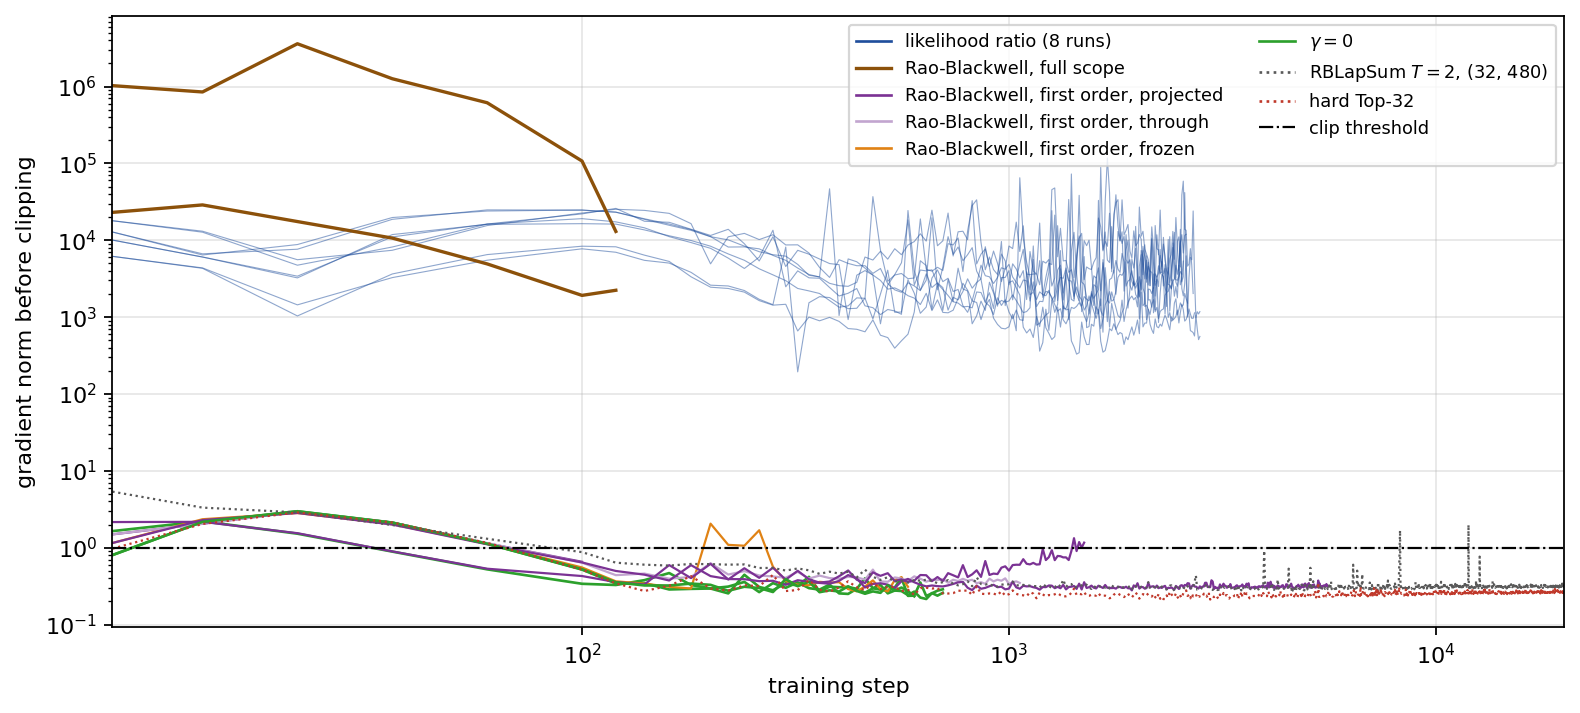
\includegraphics[width=\textwidth]{figures/policy-cr/pf_gradnorm.png}
\caption{Gradient norm before clipping against step (logarithmic norm,
step axis linear to 100 and logarithmic beyond): the eight likelihood-ratio runs
(blue), the Rao--Blackwell runs with the full scope (brown) and with the
first-order scope and the three width gradients (projected, through, frozen),
the $\gamma = 0$ controls (green), RBLapSum $T = 2$ at $(32, 480)$ and hard
Top-32 (dotted); dash-dot the clip threshold.}
\label{fig:gn}
\end{figure}

\end{document}
